\chapter{Ajuste de imagem}

O InVesalius não garante a correta ordem das imagens pois depende de informações que estão presentes nas imagens, algumas vezes essas imagens tem as informações incorretas ou não seguem o padrão DICOM. Dessa forma é recomendável confirmar se a lesão ou algum outro marco anatômico presente em um determinado paciente é exibido no lado correto da imagem. Caso não seja, é possível utilizar as ferramentas de espelhar a imagem ou inverter eixos. Também para o alinhamento da imagem, existe a ferramenta de rotação da imagem.

\section{Espelhar}

É possível espelhar um dos lados da imagem de modo que eles se invertam, para isso é necessário ir no menu, \textbf{Ferramentas}, \textbf{Imagem}, \textbf{Espelhar} e clicar em uma das seguintes opções (figura~\ref{fig:menu_img_mirroring_axis_pt}):

\begin{itemize}
	\item Direita - Esquerda
	\item Anterior - Posterior
	\item Superior - Inferior
\end{itemize}

\begin{figure}[!htb]
\centering
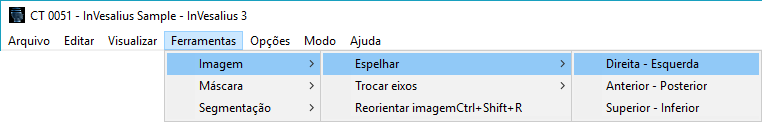
\includegraphics[scale=0.4]{menu_img_mirroring_axis_pt.png}
\caption{Menu para ativar ferramenta de espelhar imagem.}
\label{fig:menu_img_mirroring_axis_pt}
\end{figure}


A figura~\ref{fig:mirrored} apresenta um comparativo entre a imagem não espelhada e a imagem espelhada. Por o conjunto de imagens formar um volume, ao aplicar espelhamento todas as outras orientações são modificadas também.

\begin{figure}[!htb]
  \centering
  \subfloat[Imagem entrada]{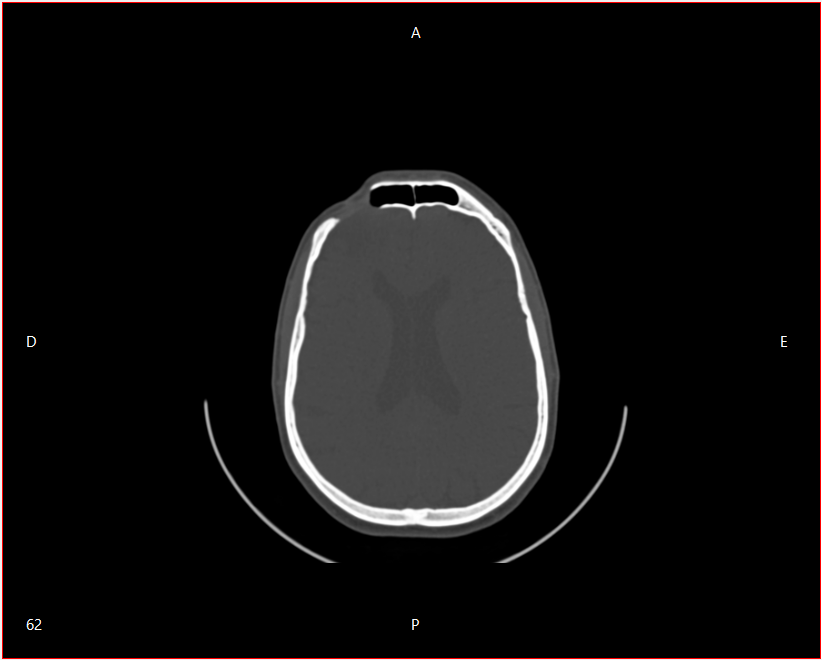
\includegraphics[width=0.45\textwidth]{mirror_axial.png}}  \qquad
  \subfloat[Imagem espelhada]{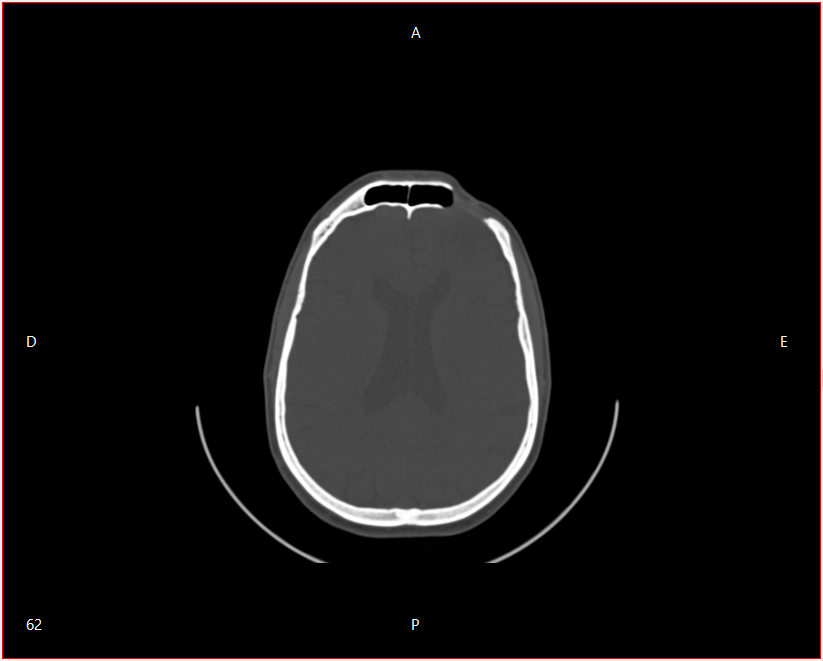
\includegraphics[width=0.45\textwidth]{mirror_axial_mirrored.png}}
  \hfill
  \caption{Exemplo de imagem com direita-esquerda espelhada.}
  \label{fig:mirrored}
\end{figure}

\section{Trocar Eixo}

A ferramenta de troca de eixo, muda as orientações da imagem caso ela tem sido importada erroneamente. Para isso é necessário ir no menu, \textbf{Ferramentas}, \textbf{Imagem}, \textbf{Trocar Eixo} e clicar em uma das seguintes opções (figura~\ref{fig:menu_invert_axis}):

\begin{itemize}
	\item Da Direita para Anterior-Posterior
	\item Da Direita-Esquerda para Superior-Inferior
	\item Da Anterior-Posterior para Superior-Inferior
\end{itemize}


As figuras~\ref{fig:invert_axis_axial} e~\ref{fig:invert_axis_axial_inverted}, apresentam um exemplo de imagens com eixo invertido.

\begin{figure}[!htb]
\centering
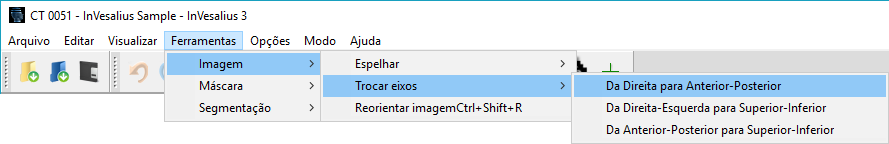
\includegraphics[scale=0.4]{menu_invert_axis_pt.png}
\caption{Menu para ativar espelhar um dos lados da imagem.}
\label{fig:menu_invert_axis}
\end{figure}

\begin{figure}[!htbp]
\centering
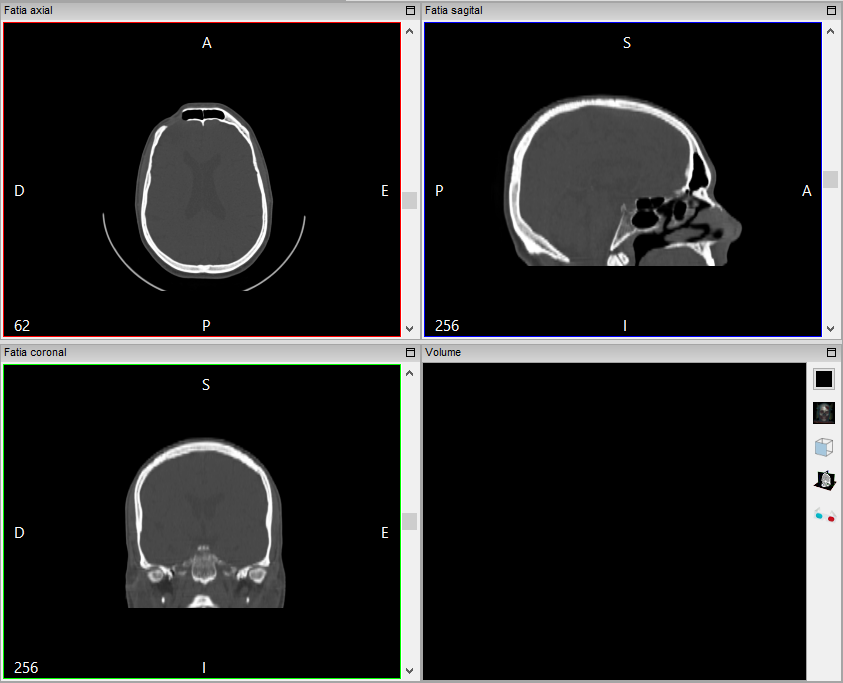
\includegraphics[scale=0.4]{invert_axis_axial_pt.png}
\caption{Conjunto de imagens antes de inverter eixo - Da Anterior-Posterior para Superior-Inferior.}
\label{fig:invert_axis_axial}
\end{figure}

\begin{figure}[!htbp]
\centering
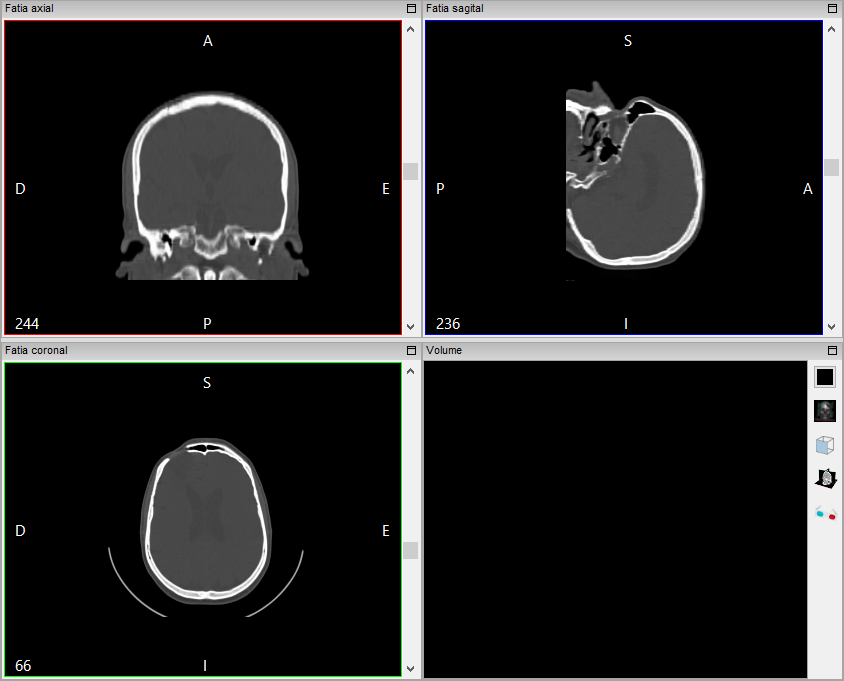
\includegraphics[scale=0.4]{invert_axis_axial_inverted_pt.png}
\caption{Conjunto de imagens com eixo invertido - Da Anterior-Posterior para Superior-Inferior.}
\label{fig:invert_axis_axial_inverted}
\end{figure}

\section{Reorientar imagem (Rotacionar)}

Caso seja necessário alinhar a imagem levando em consideração algum ponto de referencia como algum marco anatômico, é possível realizar essa tarefa utilizando a ferramenta de reorientação de imagem. Para abrir a ferramenta é necessário ir ao menu, \textbf{Ferramentas}, \textbf{Imagem} e por último \textbf{Reorientar imagem} (figura~\ref{fig:menu_img_reorient}).

\begin{figure}[!htbp]
\centering
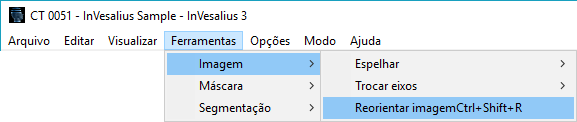
\includegraphics[scale=0.4]{menu_img_reorient_pt.png}
\caption{Menu para ativar o recurso de reorientar imagem.}
\label{fig:menu_img_reorient}
\end{figure}

Ao abrir a ferramenta será exibida uma janela (figura~\ref{fig:image_reorient_window}) que mostra em qual orientação e quantos graus a imagem foi rotacionada.

\begin{figure}[!htbp]
\centering
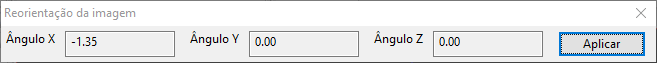
\includegraphics[scale=0.65]{image_reorient_window_pt.png}
\caption{Janela responsável por exibir os parâmetros de reorientação de imagem.}
\label{fig:image_reorient_window}
\end{figure}

\newpage

Inicialmente é necessário definir qual o método de interpolação que será aplicado ao rotacionar a imagem, por padrão o método é o tricúbico. As outras opções de interpolação são:

\begin{itemize}
	\item Vizinho mais próximo
	\item Trilinear
	\item Tricúbica
	\item Lanczos
\end{itemize}

Após selecionado o método de interpolação, é necessário definir em função de qual ponto a imagem será rotacionada, para isso é necessário \textbf{manter o botão esquerdo do mouse pressionado} entre a interseção de duas linhas (figura~\ref{fig:image_reorient_adjust_center}) em uma das janelas de orientação axial, coronal ou sagital e arrastar até o ponto desejado.

\begin{figure}[!htbp]
\centering
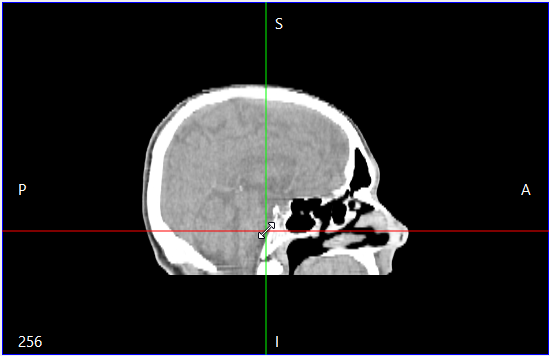
\includegraphics[scale=0.4]{image_reorient_adjust_center.png}
\caption{Definição do eixo de rotação da imagem.}
\label{fig:image_reorient_adjust_center}
\end{figure}

Para rotacionar a imagem é necessário \textbf{manter o botão esquerdo do mouse pressionado} e \textbf{arrastar} de forma que o ponto de referencia ou marco anatômico fique alinhado com uma das linhas (figura~\ref{fig:image_reorient_rotated}). Após a imagem estar na posição desejada, é necessário clicar no botão \textbf{Aplicar}, presente na janela de parâmetros (figura~\ref{fig:image_reorient_window}), dependo do tamanho da imagem é necessário aguardar alguns segundos até o processo finalizar. A figura~\ref{fig:image_reorient_rotated_applied} apresenta uma imagem com o processo de de reorientação finalizada.

\begin{figure}[!htb]
\centering
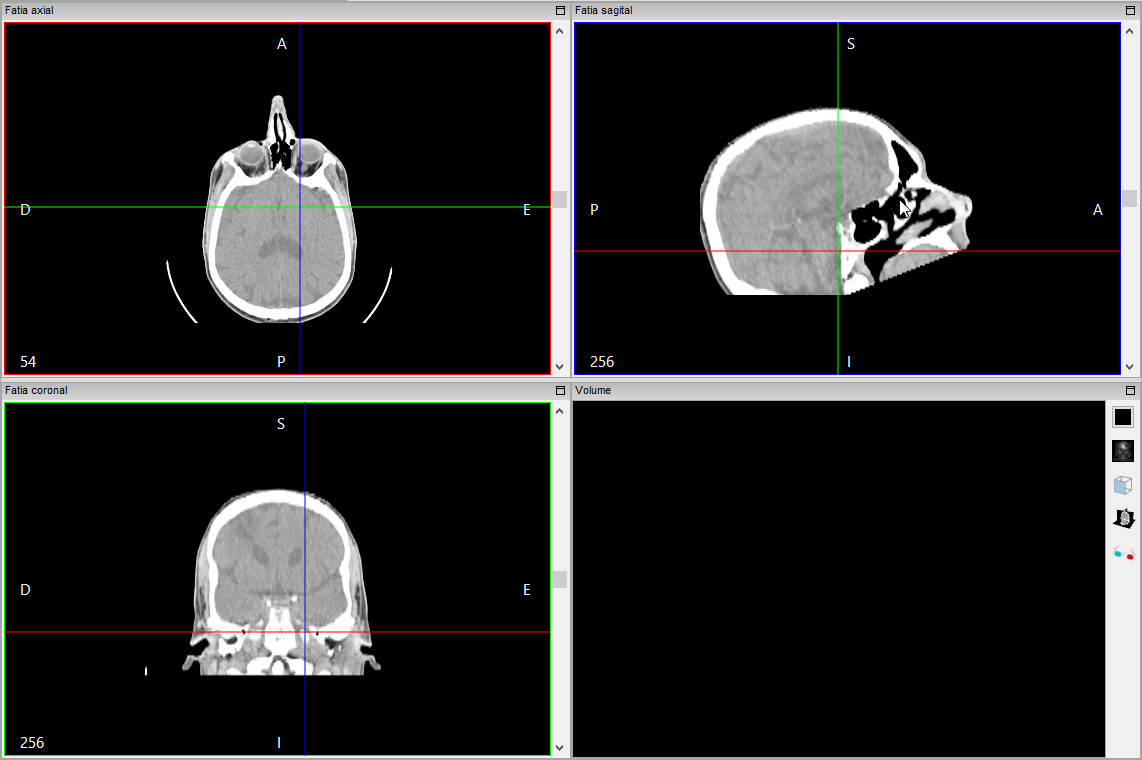
\includegraphics[scale=0.4]{image_reorient_rotated_pt.png}
\caption{Imagem rotacionada.}
\label{fig:image_reorient_rotated}
\end{figure}

\begin{figure}[!htb]
\centering
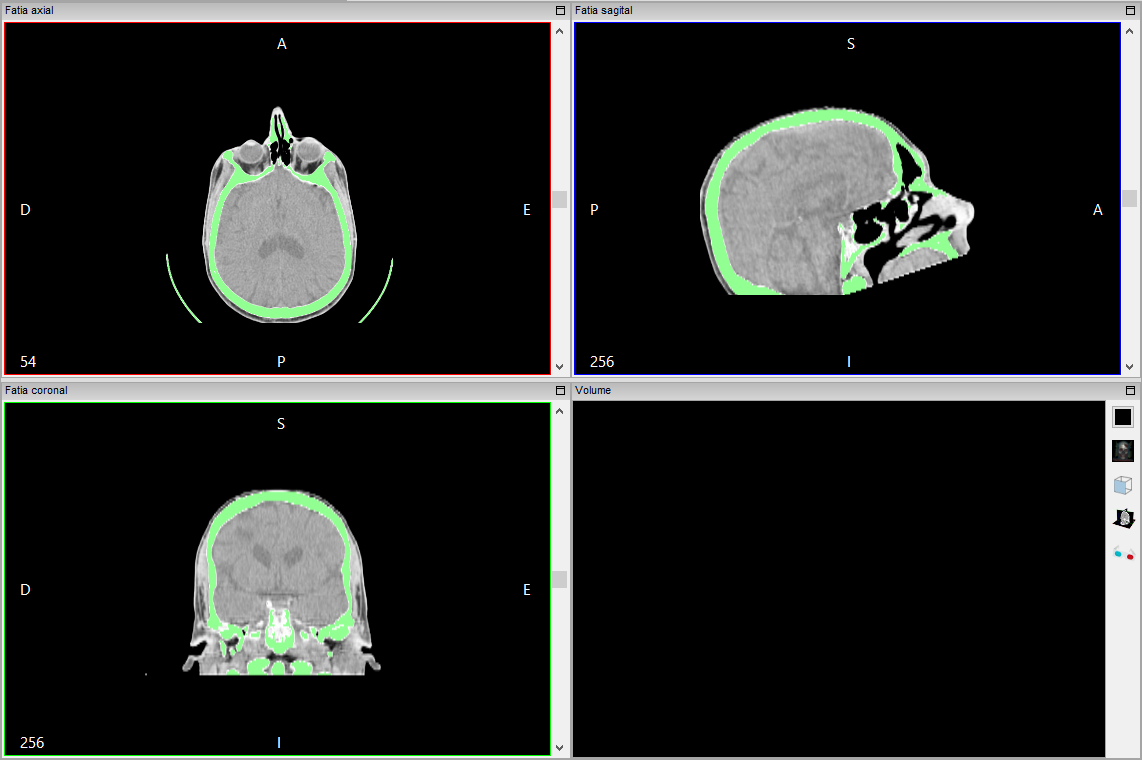
\includegraphics[scale=0.4]{image_reorient_rotated_applied_pt.png}
\caption{Imagem rotacionada após a finalização do processo.}
\label{fig:image_reorient_rotated_applied}
\end{figure}
